\documentclass[bluish,slideColor,colorBG,pdf]{prosper}
\hypersetup{pdfpagemode=FullScreen}
\usepackage{graphicx}
\def\baselinestretch{1.0}
\setlength{\topmargin}{-60pt}
\setlength{\textheight}{460pt}
\setlength{\oddsidemargin}{0pt}
\setlength{\evensidemargin}{0pt}
\setlength{\textwidth}{660pt}
\setlength{\footskip}{0pt}
\parindent 0.3in
\hyphenpenalty=10000
\tolerance=10000
\pagestyle{empty}

\def\Prob{{\rm Prob\;}}
\def\prob{{\rm \;Prob\;}}

\title{Week 2:  Searching for trees, ancestral states}
\author{Genome 570}
\institution{January, 2016}

\begin{document}

\maketitle

\begin{slide}[Replace]{Greedy search for a maximum}

\centerline{\includegraphics[width=3.5in]{fig4-1aa.ydraw}}
\bigskip

Parsimony methods search for a minimum.  The surface is easier to see if we
turn it upside down and search for a maximum.  From an arbitrary starting point ...`

\end{slide}

\begin{slide}[Replace]{Greedy search for a maximum}

\centerline{\includegraphics[width=3.5in]{fig4-1a.ydraw}}
\bigskip

If we look at the neighboring points, and ...

\end{slide}

\begin{slide}[Replace]{Greedy search for a maximum}

\centerline{\includegraphics[width=3.5in]{fig4-1b.ydraw}}
\bigskip

... then move to the highest one ...

\end{slide}

\begin{slide}[Replace]{Greedy search for a maximum}

\centerline{\includegraphics[width=3.5in]{fig4-1c.ydraw}}
\bigskip

... looking at the neighboring points, and ...

\end{slide}

\begin{slide}[Replace]{Greedy search for a maximum}

\centerline{\includegraphics[width=3.5in]{fig4-1d.ydraw}}
\bigskip

... then moving to the highest one,

\end{slide}

\begin{slide}[Replace]{Greedy search for a maximum}

\centerline{\includegraphics[width=3.5in]{fig4-1e.ydraw}}
\bigskip

... looking at the neighboring points, and ...

\end{slide}

\begin{slide}[Replace]{Greedy search for a maximum}

\centerline{\includegraphics[width=3.5in]{fig4-1f.ydraw}}
\bigskip

... then moving to the highest one,

\end{slide}

\begin{slide}[Replace]{Greedy search for a maximum}

\centerline{\includegraphics[width=3.5in]{fig4-1g.ydraw}}
\bigskip

... looking at the neighboring points, and ...

\end{slide}

\begin{slide}[Replace]{Greedy search for a maximum}

\centerline{\includegraphics[width=3.5in]{fig4-1h.ydraw}}
\bigskip

... then moving to the highest one,

\end{slide}

\begin{slide}[Replace]{Greedy search for a maximum}

\centerline{\includegraphics[width=3.5in]{fig4-1i.ydraw}}
\bigskip

... looking at the neighboring points, and ...

\end{slide}

\begin{slide}[Replace]{Greedy search for a maximum}

\centerline{\includegraphics[width=3.5in]{fig4-1j.ydraw}}
\bigskip

... then moving to the highest one,

\end{slide}

\begin{slide}[Replace]{Greedy search for a maximum}

\centerline{\includegraphics[width=3.5in]{fig4-1k.ydraw}}
\bigskip

... looking at the neighboring points, and ...

\end{slide}

\begin{slide}[Replace]{Greedy search for a maximum}

\centerline{\includegraphics[width=3.5in]{fig4-1l.ydraw}}
\bigskip

... then moving to the highest one,

\end{slide}

\begin{slide}[Replace]{Greedy search for a maximum}

\centerline{\includegraphics[width=3.5in]{fig4-1m.ydraw}}
\bigskip

... until, looking at the neighboring points, we find none that are better ...

\end{slide}

\begin{slide}[Replace]{Greedy search for a maximum}

\centerline{\includegraphics[width=3.5in]{fig4-1n.ydraw}}
\bigskip

... so we stop there, ...

\end{slide}

\begin{slide}[Replace]{Greedy search for a maximum}

\centerline{\includegraphics[width=3.5in]{fig4-1o.ydraw}}
\bigskip

... we will find better points ... 

\end{slide}

\begin{slide}[Replace]{Greedy search for a maximum}

\centerline{\includegraphics[width=3.5in]{fig4-1p.ydraw}}
\bigskip

... but not necessarily the overall best point.

\end{slide}

\begin{slide}[Replace]{Nearest-neighbor interchange (NNI)  rearrangements}

\centerline{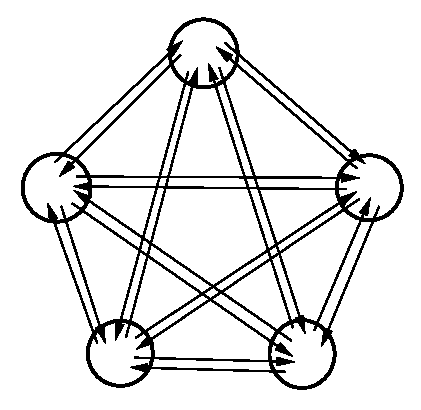
\includegraphics[width=2.5in]{fig4-2.ydraw}}

\end{slide}

\begin{slide}[Replace]{The Schoenberg graph}

\hspace*{0in}\hspace{-0.1in}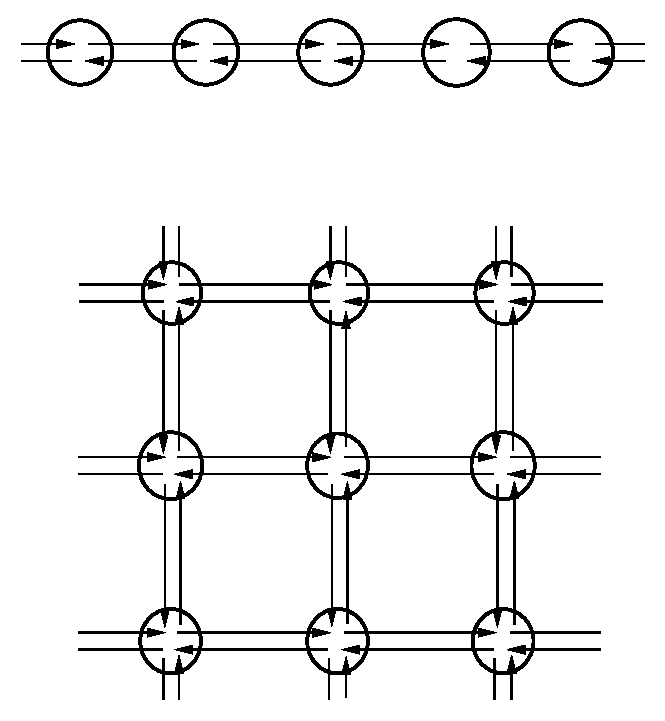
\includegraphics[width=3.2in]{fig4-3.ydraw} \hspace{-0.3in}
\parbox[b]{1.6in}{
\begin{flushleft}All 15 unrooted 5-species trees, connected if a Nearest-Neighbor
Interchange can take you from one to the other.\\
~\\
(This arrangement of the graph is due to Ben Schoenberg).
\end{flushleft}}

\end{slide}

\begin{slide}[Replace]{With numbers of steps of trees}

\hspace*{0in}\hspace{-0.1in}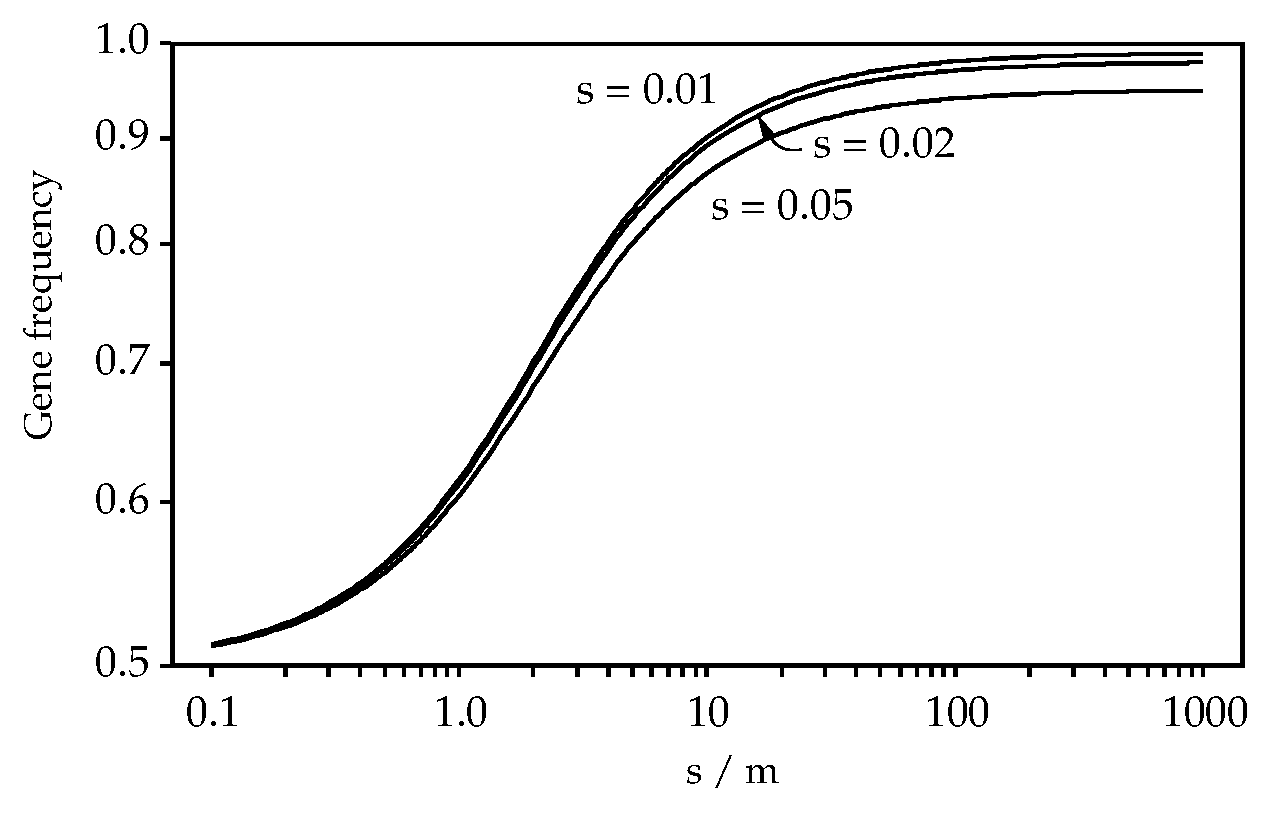
\includegraphics[width=3.2in]{fig4-4.ydraw}

\end{slide}

\begin{slide}[Replace]{Subtree pruning and regrafting (SPR) }

\centerline{\includegraphics[width=2.8in]{fig4-5a.ydraw}}

\end{slide}

\begin{slide}[Replace]{Subtree pruning and regrafting }

\centerline{\includegraphics[width=2.8in]{fig4-5b.ydraw}}

\end{slide}

\begin{slide}[Replace]{Subtree pruning and regrafting}

\centerline{\includegraphics[width=2.8in]{fig4-5c.ydraw}}

\end{slide}

\begin{slide}[Replace]{Subtree pruning and regrafting}

\centerline{\includegraphics[width=2.8in]{fig4-5d.ydraw}}

\end{slide}

\begin{slide}[Replace]{Subtree pruning and regrafting}

\centerline{\includegraphics[width=2.8in]{fig4-5e.ydraw}}

\end{slide}

\begin{slide}[Replace]{Subtree pruning and regrafting}

\centerline{\includegraphics[width=2.8in]{fig4-5f.ydraw}}

\end{slide}

\begin{slide}[Replace]{Tree bisection and reconnection (TBR) } 

\centerline{\includegraphics[width=3in]{fig4-6a.ydraw}}

\end{slide}

\begin{slide}[Replace]{Tree bisection and reconnection}

\centerline{\includegraphics[width=3in]{fig4-6b.ydraw}}

\end{slide}

\begin{slide}[Replace]{Tree bisection and reconnection}

\centerline{\includegraphics[width=3in]{fig4-6c.ydraw}}

\end{slide}

\begin{slide}[Replace]{Tree bisection and reconnection}

\centerline{\includegraphics[width=3in]{fig4-6d.ydraw}}

\end{slide}

\begin{slide}[Replace]{Tree bisection and reconnection}

\centerline{\includegraphics[width=3in]{fig4-6f.ydraw}}

\end{slide}

\begin{slide}[Replace]{Tree bisection and reconnection}

\centerline{\includegraphics[width=3in]{fig4-6g.ydraw}}

\end{slide}

\begin{slide}[Replace]{Goloboff's economy in rearranging}

\centerline{\includegraphics[width=3.5in]{fig4-7.ydraw}}
\bigskip

If we compute the relevant interior arrays of steps beyond that point in the 
tree, we can very quickly evaluate different reconnections of the two parts of the tree.


\end{slide}

\begin{slide}[Replace]{Sequential addition}

\centerline{\includegraphics[width=2.8in]{fig4-8.ydraw}}

\end{slide}

\begin{slide}[Replace]{Star decomposition}

\centerline{\includegraphics[width=4.2in]{fig4-9.ydraw}}

\end{slide}

\begin{slide}[Replace]{Some cleverer rearrangement methods}

\begin{itemize}
\item Kevin Nixon's ``parsimony ratchet'' search ({\it Cladistics}, 1999).
This samples subsets of characters, uses just those characters in heuristic
search to find a tree, then evaluates the resulting tree on the full data
set.  If it is better than the previous best tree, it becomes the starting
point for more heuristic search, and more rounds of the ratchet.  This
works for other criteria other than parsimony too.
\medskip

\item Genetic algorithms.  Several researchers have made genotypes that
each describe a tree, and searched by computing a fitness from the parsimony
score of the tree, and evolving a population of trees based on mutation,
mating, selection, and recombination among these tree representation
``genotypes''.
\end{itemize}

\end{slide}

\begin{slide}[Replace]{An example of looking for the Shortest Hamiltonian path}

\centerline{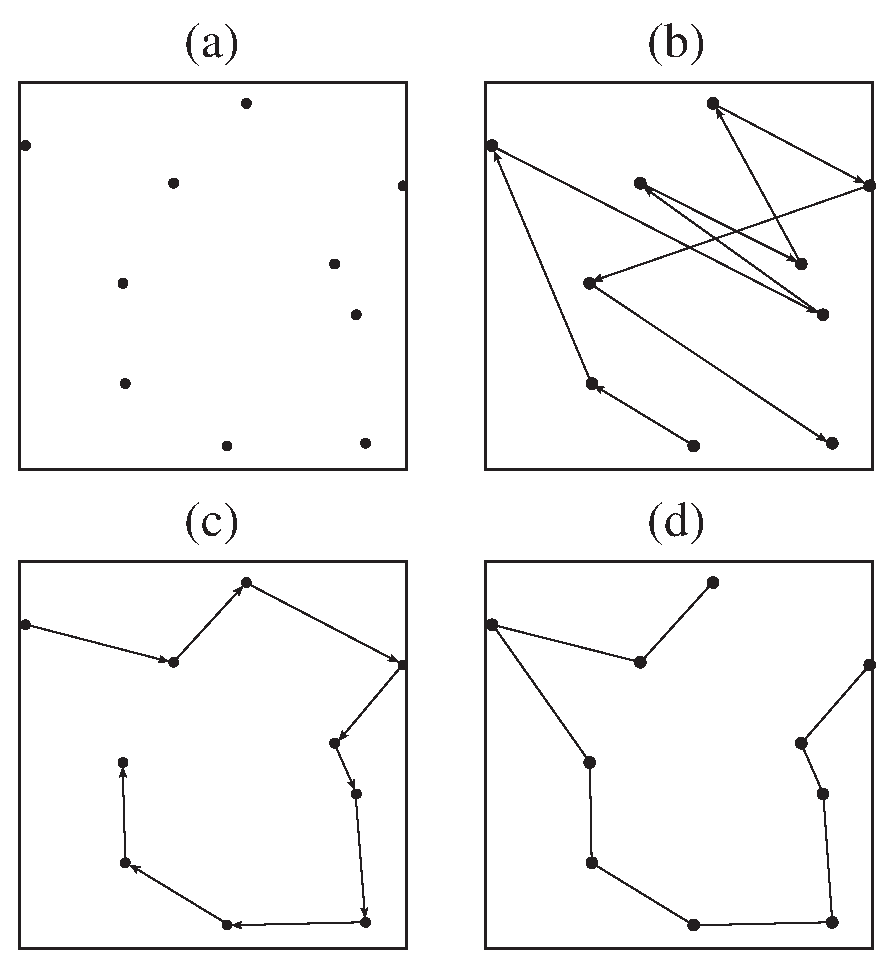
\includegraphics[width=4.0in]{fig5-1.ydraw}}

\end{slide}

\begin{slide}[Replace]{A search tree of paths}

\centerline{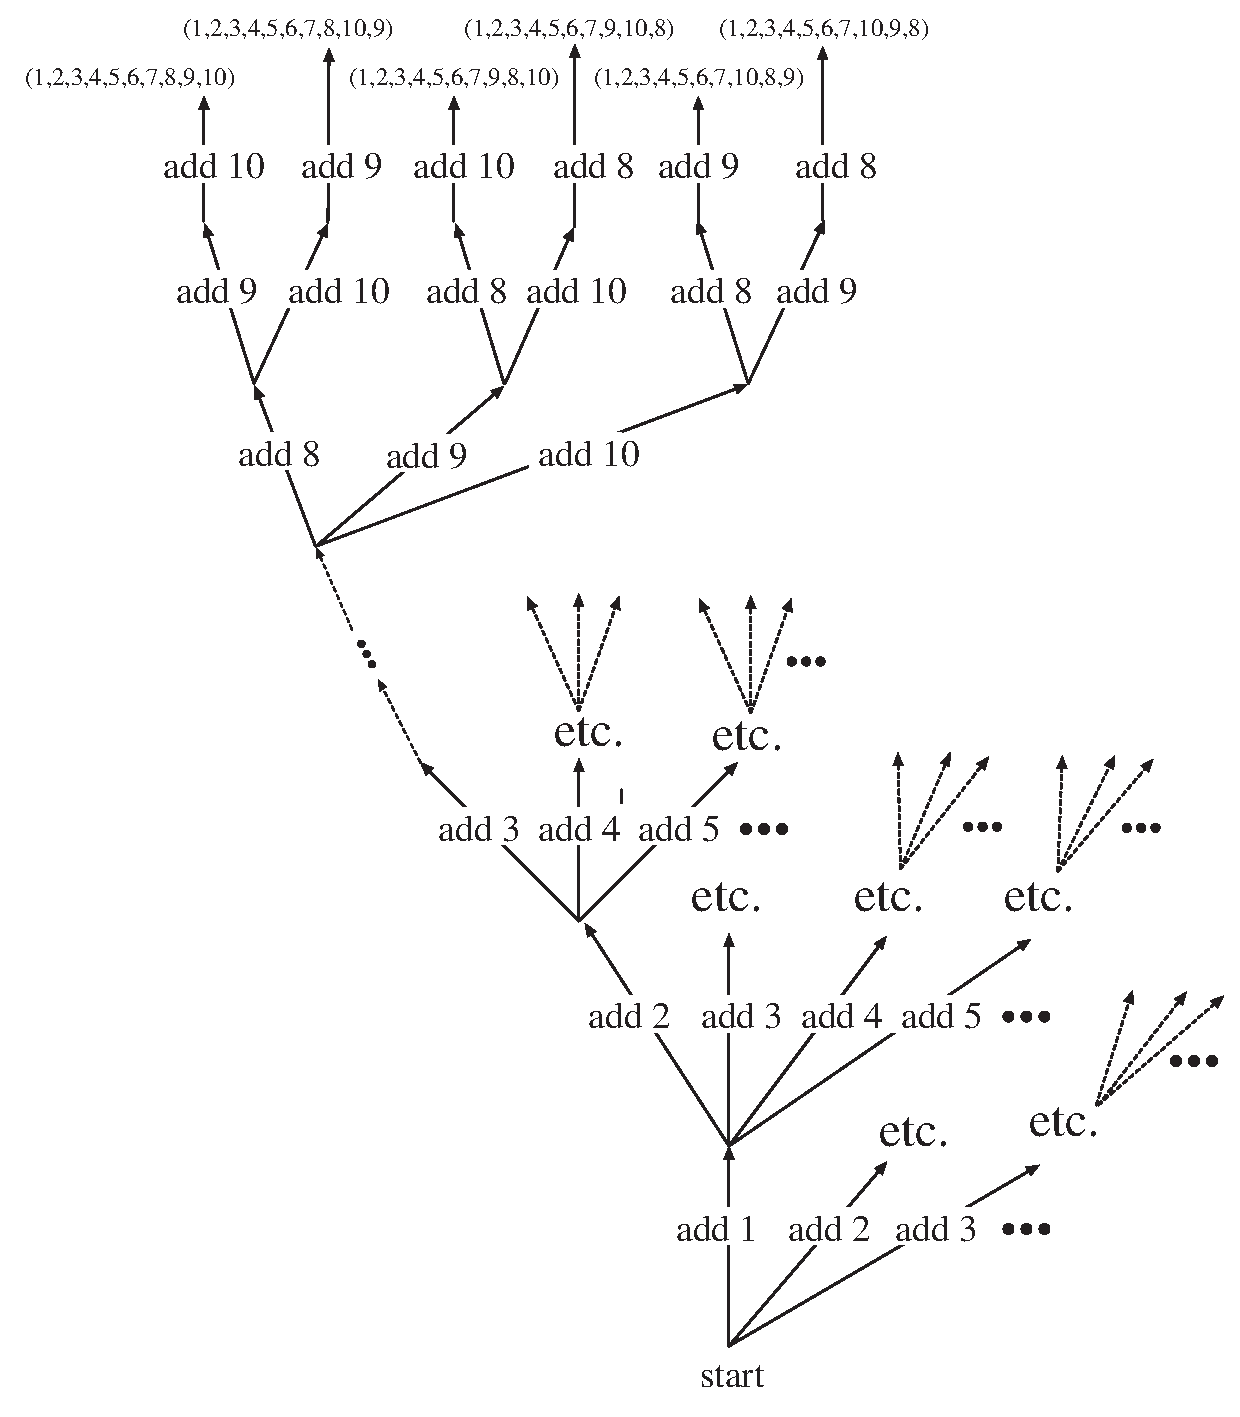
\includegraphics[width=2.8in]{fig5-2.ydraw}}

\end{slide}

\begin{slide}[Replace]{Time-savings of branch and bound}
\bigskip

Results for this case:
\bigskip

\renewcommand{\arraystretch}{1.4}
\begin{tabular}{l | r r}
Algorithm & length & time \\
\hline
Greedy search from all points & 2.802660  & (too fast to measure) \\
Exhaustive enumeration & 2.781230 & 10.85 sec \\
Branch and bound &  2.781230 & 0.46 sec
\end{tabular}


\end{slide}

\begin{slide}[Replace]{Branch and bound on trees}

\centerline{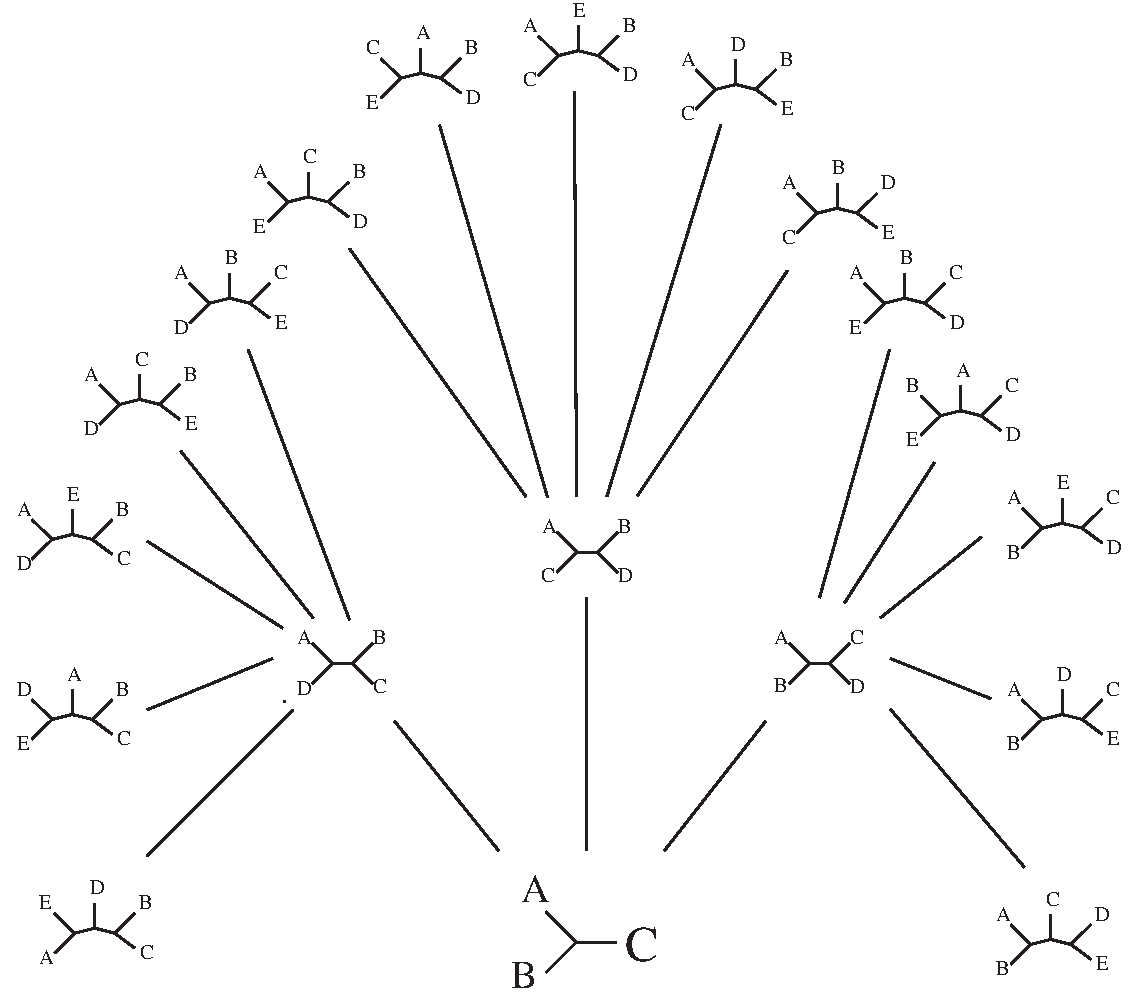
\includegraphics[width=3.2in]{fig5-3.ydraw}}

\end{slide}

\begin{slide}[Replace]{Branch and bound using numbers of steps}

\centerline{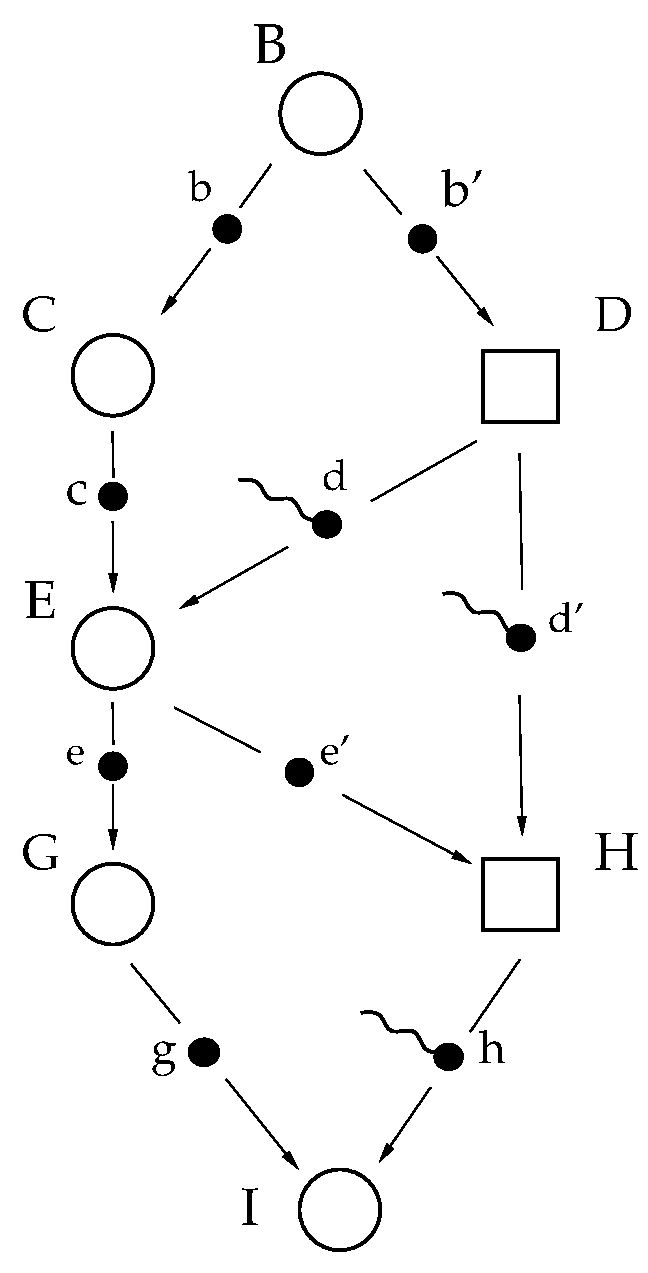
\includegraphics[width=3.2in]{fig5-4.ydraw}}

\end{slide}

\begin{slide}[Replace]{Calculating a lower bound on tree score}

\begin{itemize}
\item The score of the partial tree is a lower bound (since adding
more species cannot decrease the number of steps)
\medskip

\item Also can add the number of characters that do not show variation
on the species added so far, but will once added (actually, the number
of new states that will appear once all species are added -- if A and G
are there already, will C also appear?)
\medskip

\item Can also take all disjoint pairs of characters that will become
incompatible once added, but aren't incompatible now (this is due to
Dave Swofford.  Each brings in one more step.)
\end{itemize}

\end{slide}

\begin{slide}[Replace]{Polynomial time and exponential time}

\centerline{\includegraphics[width=2.3in]{poly.idraw}}
\bigskip

How does the time taken by an algorithm depend on the size of the
problem?  If it is a polynomial (even one with big coefficients),
with a big enough case it is faster than one that depends on the
size exponentially.

\end{slide}

\begin{slide}[Replace]{NP completeness and NP hardness}

\centerline{\includegraphics[height=1.8in]{np.ydraw}}
\bigskip

P = problems that can be solved by a polynomial time algorithm
\medskip

NP complete = problems for which a proposed solution can be checked in
polynomial time but for which it can be proven that if one of them is in
P, all of them are.
\medskip

NP hard = problems for which a solution can be checked in polynomial
time, but might be not solvable in polynomial time

\end{slide}

\begin{slide}[Replace]{Inferring ancestor at the root of the tree}

\centerline{\includegraphics[width=4in]{fig2-2.idraw}}
\bigskip

\end{slide}

\begin{slide}[Replace]{Parsimony reconstruction of ancestral states}

\centerline{\includegraphics[width=2.2in]{fig6-1.ydraw}}
\bigskip

Given the reconstruction in an ancestor, choosing the most parsimonious one in
one of its descendants.

\end{slide}

\begin{slide}[Replace]{Ancestral states in the example}

\centerline{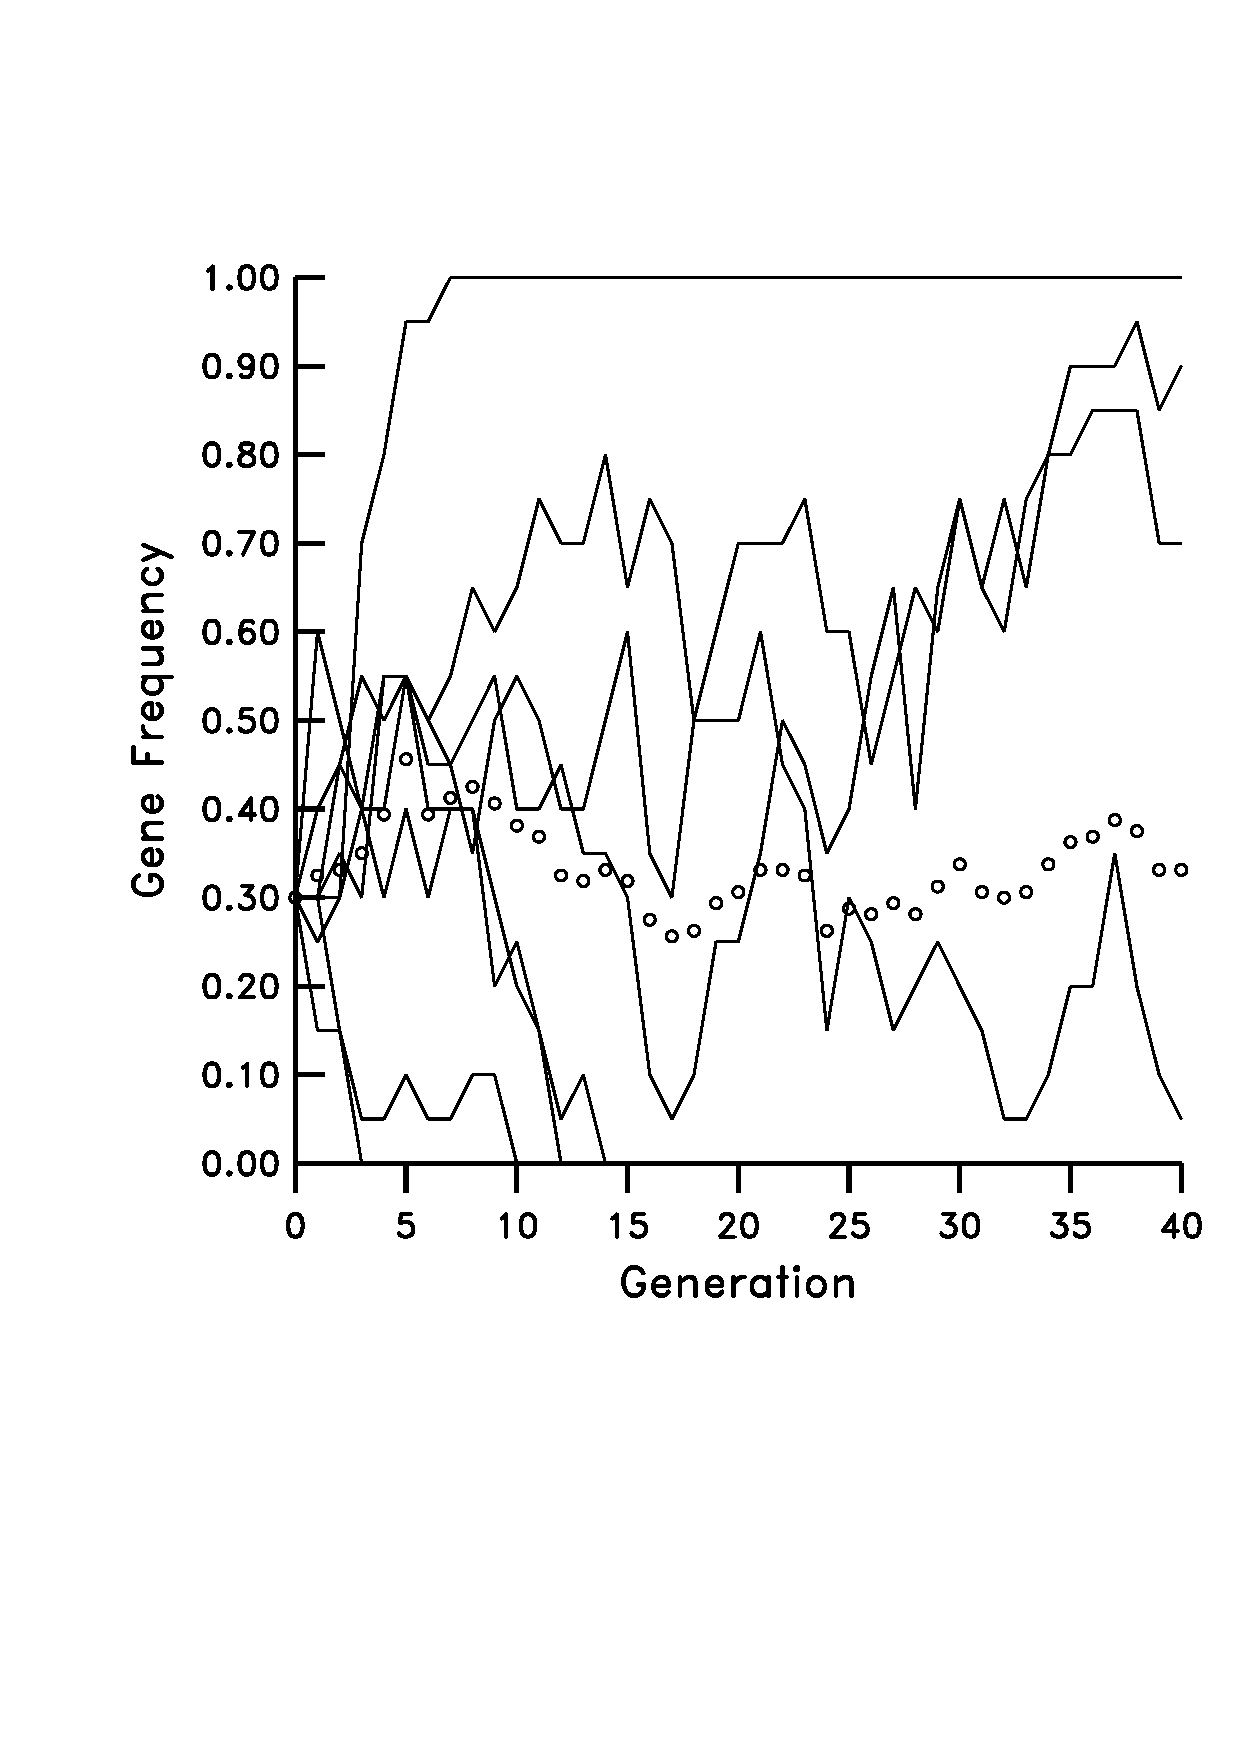
\includegraphics[width=4in]{fig6-2.ydraw}}

\end{slide}

\begin{slide}[Replace]{One reconstruction}

\centerline{\includegraphics[width=4in]{fig6-2a.ydraw}}

\end{slide}

\begin{slide}[Replace]{For the other choice, two possibilities}

\centerline{\includegraphics[width=4in]{fig6-2b.ydraw}}

\end{slide}

\begin{slide}[Replace]{One of these}

\centerline{\includegraphics[width=4in]{fig6-2c.ydraw}}

\end{slide}

\begin{slide}[Replace]{The other one}

\centerline{\includegraphics[width=4in]{fig6-2d.ydraw}}

\end{slide}

\begin{slide}[Replace]{There can be multiple tied reconstructions}

\centerline{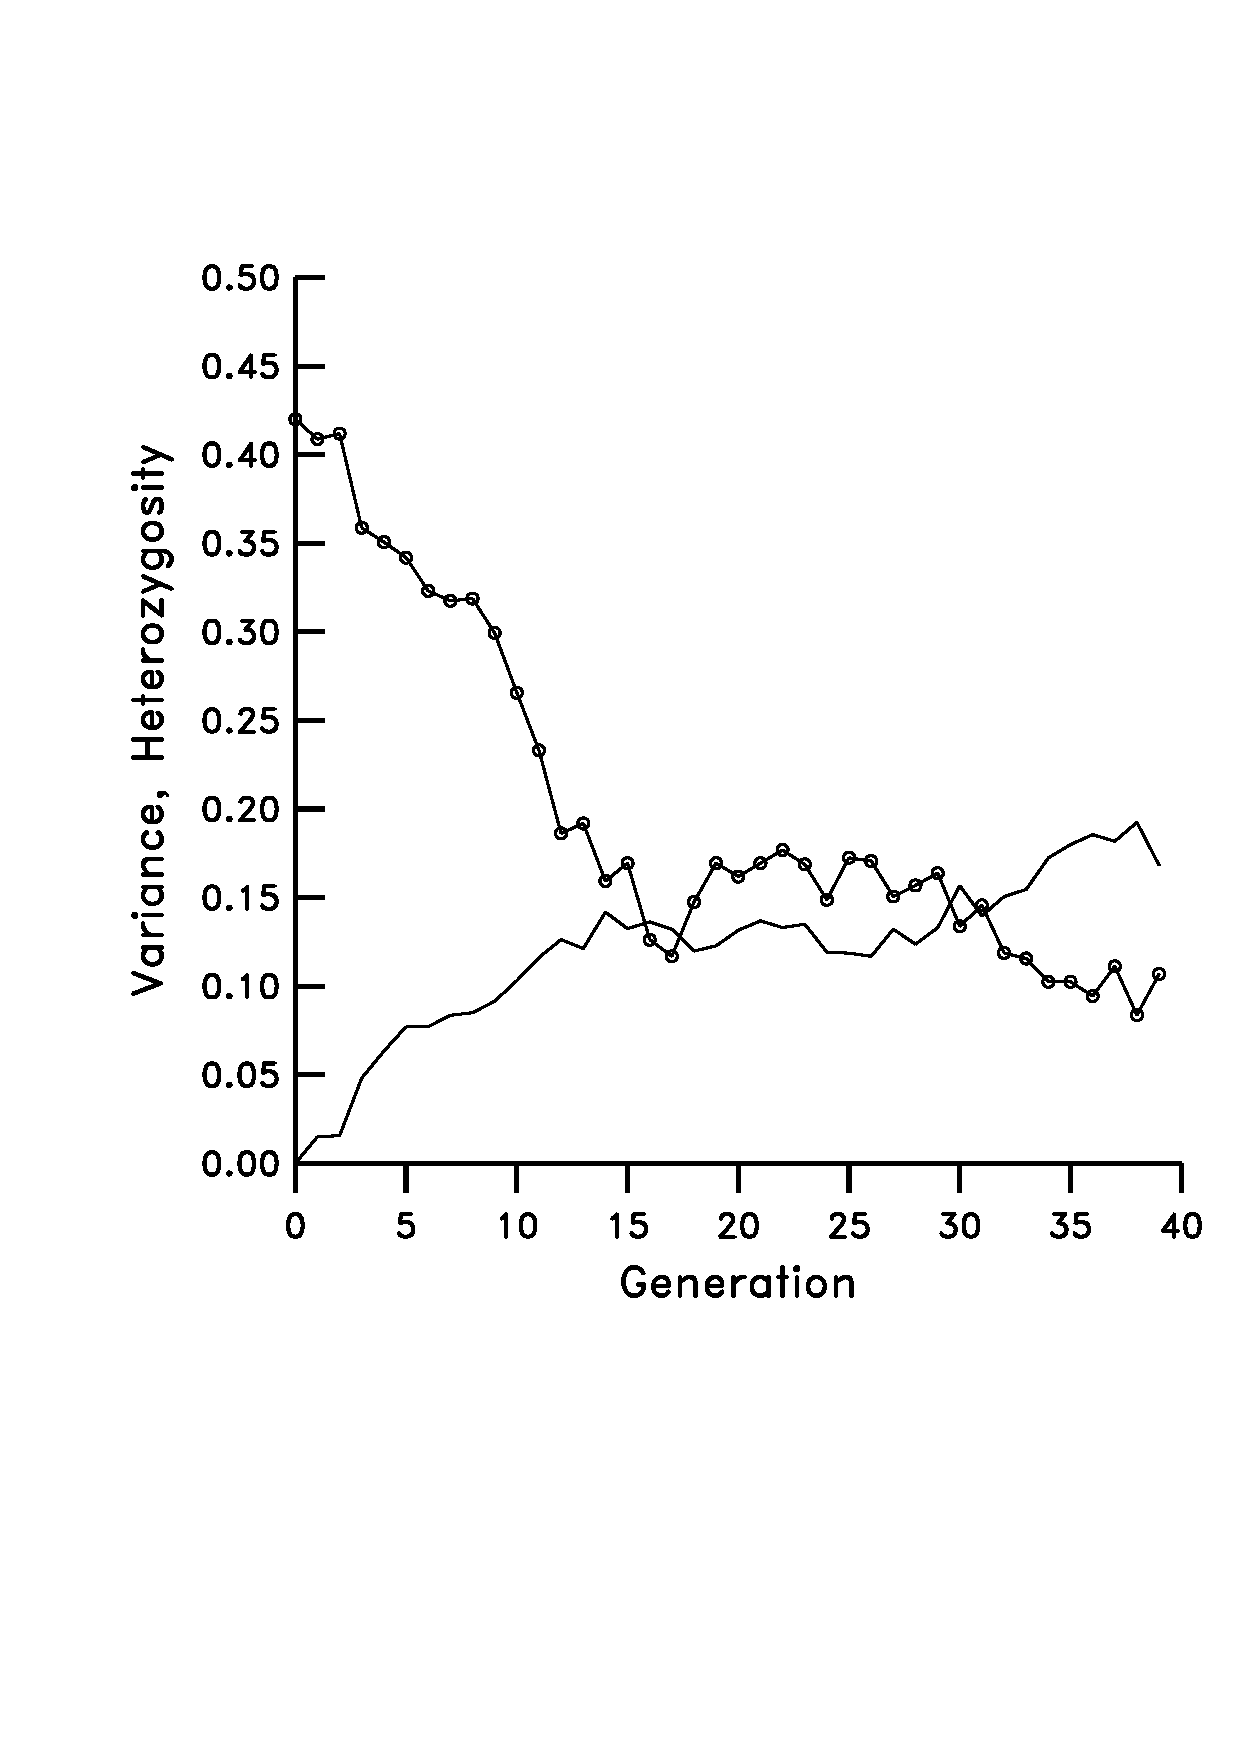
\includegraphics[width=3in]{fig6-3.ydraw}}

\end{slide}

\begin{slide}[Replace]{Average branch lengths over all reconstructions}

\centerline{\includegraphics[width=3.4in]{fig6-4.ydraw}}

\end{slide}

\begin{slide}[Replace]{Camin-Sokal parsimony}

\centerline{\includegraphics[width=2.5in]{fig7-1.ydraw}}
\bigskip

Unidirectional change.  Easy to reconstruct ancestors and count states.  This
scheme is of importance in comparative genomics, with 1 = presence of a
deletion.

\end{slide}

\begin{slide}[Replace]{Dollo parsimony}

\centerline{\includegraphics[width=2.5in]{fig7-2.ydraw}}
\bigskip

Assumes that it is much more difficult to gain state 1 than to lose it.
Has been used to model gain and loss of restriction sites.

\end{slide}

\begin{slide}[Replace]{Polymorphism parsimony}

\centerline{\includegraphics[width=3.0in]{fig7-3.ydraw}}
\bigskip

Note that in this case the retention (not the loss) of the polymorphic state 
(01) is considered unlikely and is penalized.

\end{slide}

\begin{slide}[Replace]{nonadditive binary coding}

\centerline{\includegraphics[width=3.5in]{fig7-4.ydraw}}
\bigskip

Using multiple 0/1 characters to construct a case with the same parsimony
score on all trees as a single multistate character with a ``character state
tree''

\end{slide}

\begin{slide}[Replace]{Dollo parsimony -- a paradox}

\centerline{\includegraphics[width=4in]{fig7-5.ydraw}}
\bigskip

With a character-state tree, can you always find a Dollo parsimony
reconstruction that has only one origin of state 2 ?

\end{slide}

\end{document}

